\documentclass[11pt]{article}
\usepackage[a4paper,margin=1in]{geometry}
\usepackage[T1]{fontenc}
\usepackage{lmodern,microtype}
\usepackage{amsmath,amssymb,amsthm}
\usepackage{booktabs,tabularx,multirow}
\usepackage{graphicx,xcolor}
\usepackage[hidelinks]{hyperref}
\usepackage{enumitem}
\setlist{nosep,leftmargin=1.4em}
\emergencystretch=3em

\newtheorem{theorem}{Theorem}
\newtheorem{lemma}{Lemma}
\newtheorem{corollary}{Corollary}
\newtheorem{proposition}{Proposition}
\newtheorem{definition}{Definition}
\theoremstyle{remark}
\newtheorem{remark}{Remark}

\newcommand{\sk}{\mathsf{sk}}
\newcommand{\vk}{\mathsf{vk}}
\newcommand{\seed}{\mathsf{seed}_{\mathsf{wallet}}}
\newcommand{\Leak}{\mathsf{Leak}}
\newcommand{\SB}{Shielded Bitcoin}
\newcommand{\sysname}{\textsf{SBEW}}

\title{\textbf{Embedded Wallets for Shielded Bitcoin}\\[4pt]
\large Threshold Seed Custody, Proving Placement, and Side-Channel-Hardened\\ PIN Authorization for Replay-Based Shielded Transfers}
\author{Roi Mateo\\ \small\texttt{roimateo.nsofts@gmail.com} \and Kiley Kunze Zhai\\ \small\texttt{zhai16263@gmail.com} \and Suzuki Motoyasu\\ \small\texttt{suzukimotoyasu9429@outlook.com}}
\date{\small November 2026}

\begin{document}
\maketitle

\begin{abstract}
\SB{} is a recently proposed metaprotocol for private Bitcoin-denominated transfers on the Bitcoin L1: value is held in encrypted notes, spends publish nullifiers, validity is established by a zero-knowledge proof, and the shielded state is reconstructed by deterministic replay of Bitcoin-published envelopes. Its specification assumes a self-contained wallet, whereas mainstream adoption increasingly runs through embedded wallets, whose keys live inside an app, are unlocked with a PIN or biometric, and are backed up by a provider. We ask how to build such a wallet without turning the provider into a custodian or a surveillance point. Two obstacles arise: spend authority is a scalar consumed as a proof witness rather than a signing key, so threshold-signature designs do not apply; and the PIN that gates key release leaks timing information to any Android app through the battery fuel gauge. We present \sysname{}, which (i) splits the wallet seed 2-of-3 across a hardware-bound device share, a provider share released by an attempt-limited oblivious-PRF PIN check, and a recovery share; (ii) defines on-device, enclave, and collaborative proving with their trust and leakage; (iii) replaces single-indexer trust with $k$-of-$n$ root agreement and delta-download synchronization; (iv) hardens PIN entry; and (v) wraps the device share on Cortex-M chips with the tweakable block cipher Rotom. We prove non-custody, PIN-leak tolerance, theft resistance, sync integrity, recovery, and the security of the Rotom wrap by reduction to the \SB{} security theorem and standard assumptions. We also prove that randomized keypads leak at most a PIN's digit-repetition pattern, capping ten-guess success on 4-digit PINs at 1.5\%, and at the blind rate for distinct digits; in simulation, fixed keypads sampled at 10\,Hz raise it from 0.1\% to 1.2--6.7\%. Finally, a provider that both scans incoming notes and relays envelopes can reconstruct its users' payment graph. \sysname{} requires no change to the \SB{} protocol.
\end{abstract}

\noindent\textbf{Keywords:} Shielded Bitcoin, embedded wallets, threshold secret sharing, oblivious PRF, zero-knowledge proofs, side channels, fuel gauge, tweakable block ciphers, Rotom

\section{Introduction}

Bitcoin's transaction graph is public. \SB{}~\cite{sb26} proposes shielded transfers that are published on Bitcoin L1 without consensus changes: a sender publishes a transfer \emph{envelope} carrying nullifiers, recipient ciphertexts, a sender-recovery ciphertext, and a succinct proof; indexers replay accepted envelopes in Bitcoin order to maintain a note tree, a nullifier set, and block-level roots. Its key hierarchy derives spend, nullifier, incoming-viewing, and outgoing-viewing capabilities from one seed, and its disclosure model guarantees that no read capability confers spend authority~\cite[§6--7]{sb26}.

The \SB{} specification is deliberately scoped to the transfer layer. It notes that a prover separated from the wallet ``is inside the sender's trusted computing base''~\cite[§10]{sb26}, that a wallet which does not replay treats its indexer as a trusted component (assumption A11)~\cite[§17]{sb26}, and it leaves wallet policy, fee publication, and network observation as future work~\cite[§22]{sb26}. These are precisely the components that an \emph{embedded wallet}---a wallet whose keys are provisioned inside a consumer app and unlocked with a short secret---must decide.

Embedded wallets are attractive because they remove seed-phrase handling from the user, but their security rests on three things that interact badly with a shielded protocol:
\begin{enumerate}
  \item \textbf{Key custody without a signature.} Current embedded wallets typically split a signing key with threshold ECDSA or Schnorr~\cite{gg18,frost20} or keep it in a provider enclave. In \SB{}, however, spending is authorized by proving knowledge of $\sk_{\mathsf{spend}}$ inside the transfer circuit, from which the circuit itself derives $\sk_{\mathsf{nf}}$ and the diversified transmission key~\cite[§9, §14]{sb26}. There is no signature to thresholdize.
  \item \textbf{Short-secret authorization on a leaky device.} The PIN that releases key material is entered on a phone. Giraud and Naccache~\cite{gn23} showed that on Android 9--12 any application can sample the battery fuel gauge's instantaneous current through \texttt{BatteryManager} without user-visible permission, detect individual key presses, and use inter-press timing to narrow the PIN candidates entered in another application.
  \item \textbf{A provider who sees a lot.} The provider authenticates the user, may scan for incoming notes, and may relay envelopes. Each role is benign alone; combined, they can undo the transfer-layer privacy that \SB{} provides.
\end{enumerate}

\paragraph{Contributions.}
\begin{itemize}
  \item A system and threat model for embedded \SB{} wallets with five adversary classes, including a co-resident malicious app exploiting the fuel-gauge channel (§\ref{sec:model}).
  \item \sysname{}, a method that maps every \SB{} capability to a custody location, splits $\seed$ 2-of-3 with an attempt-limited OPRF PIN gate, and defines three proving placements with explicit trust and leakage (§\ref{sec:method}).
  \item A synchronization procedure that replaces single-indexer trust (A11) with $k$-of-$n$ root agreement and privacy-preserving delta download (§\ref{sec:sync}).
  \item Game-based definitions and full proofs for non-custody, PIN-leak tolerance, device theft, sync integrity, and recovery; an exact, tight guessing bound for randomized keypads (Theorem~\ref{thm:rand}); and a proof that a provider using V1 with authenticated relaying reconstructs its users' payment graph (§\ref{sec:analysis}).
  \item A hardware-wallet variant that wraps the device share with Rotom-256~\cite{rotom26} under structured tweaks, with a proof of privacy and integrity (Theorem~\ref{thm:rw}), a bound on the chosen-input power traces an attacker can collect (Proposition~\ref{prop:dpa}), and cycle costs derived from the Rotom implementation figures (§\ref{sec:hw}, §\ref{sec:rwproof}).
  \item A quantitative model of fuel-gauge PIN leakage and of the effect of keypad randomization (§\ref{sec:eval}).
\end{itemize}
\sysname{} changes nothing in the \SB{} transfer relation, envelope, or replay rules; it is a wallet-layer and deployment-profile construction. A protocol-level alternative that would enable threshold signing is discussed separately (§\ref{sec:split}).

\section{Background}
\label{sec:bg}

\subsection{\SB{} wallet capabilities}
Table~\ref{tab:caps} summarizes the \SB{} key hierarchy~\cite[Table~1]{sb26}. All capabilities are derived from a uniformly random 32-byte $\seed$ with domain-separated HKDF-SHA256 labels; the specification states that low-entropy passwords are not suitable seeds~\cite[App.~A.2]{sb26}. A payment address is $(d, \mathsf{pk}_d)$ with $\mathsf{pk}_d = [\sk_{\mathsf{view}}]G_d$ and $\sk_{\mathsf{view}}$ derived from $\vk_{\mathsf{in}}$.

\begin{table}[t]
\centering\small
\begin{tabularx}{\linewidth}{@{}lXl@{}}
\toprule
Object & Derivation~\cite{sb26} & Capability \\
\midrule
$\sk_{\mathsf{master}}$ & $\mathrm{HKDF}_{\mathsf{master}}(\seed)$ & root secret \\
$\sk_{\mathsf{spend}}$ & $\mathrm{ScalarFromBytes}(\mathrm{HKDF}_{\mathsf{spend}}(\sk_{\mathsf{master}}))$ & spend authority (proof witness) \\
$\sk_{\mathsf{nf}}$ & $\mathrm{HKDF}_{\mathsf{nf}}(\sk^{\mathsf{ser}}_{\mathsf{spend}})$, re-derived in circuit & nullifier derivation \\
$\vk_{\mathsf{in}}$ & $\mathrm{HKDF}_{\mathsf{in}}(\sk^{\mathsf{ser}}_{\mathsf{spend}})$ & incoming detection, read-only \\
$\vk_{\mathsf{out}}$ & $\mathrm{HKDF}_{\mathsf{out}}(\sk_{\mathsf{master}})$ & sent-note recovery, read-only \\
\bottomrule
\end{tabularx}
\caption{\SB{} wallet capabilities. Only $\sk_{\mathsf{spend}}$ (and its ancestors) authorizes spends.}
\label{tab:caps}
\end{table}

A spend proves, for each input, Merkle membership under a replayed anchor root $R[h_{\mathsf{anchor}}]$, correct nullifier derivation $\mathsf{nf} = H_{\mathsf{nf}}(\sk_{\mathsf{nf}}, \rho, \mathsf{pos})$, and the ownership rule that re-derives $\mathsf{pk}_d$ from $\sk_{\mathsf{spend}}$; it also proves ciphertext consistency and value conservation, and binds the whole body through $h_{\mathsf{body}}$~\cite[§13--14]{sb26}. The witness contains note plaintexts, Merkle paths, and a single $\sk_{\mathsf{spend}}$ for all inputs~\cite[§14.3]{sb26}. The reference profile uses Groth16, a 2-input/2-output envelope of 610 bytes in one \texttt{OP\_RETURN} output, and an anchor window of $W{=}100$, $K_{\min}{=}1$ blocks~\cite[App.~A]{sb26}.

Two specification statements constrain any wallet architecture. A delegated prover is in the sender's TCB because it sees the witness~\cite[§10]{sb26}. A wallet that does not verify replay must trust its indexer for the claimed prefix (A11)~\cite[§17]{sb26}. The privacy theorem covers the accepted-transfer transcript; fee linkage, network observation, and wallet policy are outside it and are characterized as additional leakage~\cite[§20]{sb26}.

\subsection{Embedded wallets}
We use \emph{embedded wallet} for any wallet whose key material is created and used inside a host application, unlocked with a short user secret (PIN, passkey, biometric), and recoverable through a provider-assisted flow without a user-managed seed phrase. Deployed designs combine three ingredients: hardware-bound device keys (Android Keystore/StrongBox, Apple Secure Enclave); provider-held key shares, either for threshold signing~\cite{gg18,frost20} or released after short-secret authentication; and attempt-limited PIN verification in an HSM or enclave, typically built on an oblivious PRF so that the server never sees the PIN~\cite{opaque18}. Attempt limiting is what makes a 4- or 6-digit PIN meaningful: an attacker without the provider's cooperation gets at most $L$ online guesses.

\subsection{The fuel-gauge side channel}
Giraud and Naccache~\cite{gn23} observe that high-end Android devices delegate battery accounting to a dedicated fuel-gauge IC whose \texttt{CURRENT\_NOW} reading is exposed to every application via \texttt{BatteryManager}, with no SELinux, framework, or runtime restriction on Android~12 and earlier. The register refreshes at roughly 4--10\,Hz, too slow for cryptographic side channels but fast enough for human input. A foreground service (permission granted without a prompt) can sample in the background. Touches are visible as current spikes, sharply so when haptic feedback is enabled. Using the time between presses and the known position of the confirmation key, the authors enumerate PINs consistent with the observed delays by walking backwards from the validation key. They do not quantify success rates. For an embedded wallet, this channel attacks exactly the secret that gates key release.

\section{System and Threat Model}
\label{sec:model}

\paragraph{Parties.} The user's device $\mathcal{D}$ runs the host app and has a hardware keystore offering non-exportable, app-scoped keys with optional user-presence (biometric) gating. In the hardware variant (§\ref{sec:hw}), the device share is instead held by a microcontroller with a chip-unique key. The provider $\mathcal{P}$ authenticates the user, runs an HSM or attested enclave that stores one seed share and enforces a PIN attempt counter, and may optionally offer note scanning, proving, and relaying. Indexers $\mathcal{I}_1,\dots,\mathcal{I}_n$ replay \SB{} and serve roots, leaves, and nullifiers; they are operated by parties independent of $\mathcal{P}$ and of each other. A recovery channel $\mathcal{R}$ (a passkey-protected backup or offline card) holds the third share.

\paragraph{Adversaries.}
\begin{description}[leftmargin=1em,style=nextline]
  \item[$\mathsf{A}_{\mathsf{app}}$ --- co-resident malicious app.] Runs on $\mathcal{D}$ under a different UID, can sample the fuel gauge and other zero-permission sensors, cannot read other apps' memory or use their keystore keys.
  \item[$\mathsf{A}_{\mathsf{thief}}$ --- device thief.] Physically holds an unlocked or locked $\mathcal{D}$; may also hold a fuel-gauge trace collected earlier by $\mathsf{A}_{\mathsf{app}}$.
  \item[$\mathsf{A}_{\mathsf{prov}}$ --- malicious or breached provider.] Controls $\mathcal{P}$'s storage and logic outside the HSM. It does not collude with the device or with the holder of the recovery share: any two shares reconstruct the seed, so no 2-of-3 scheme can tolerate such collusion.
  \item[$\mathsf{A}_{\mathsf{idx}}$ --- dishonest indexers.] Up to $t$ of the $n$ indexers return arbitrary roots, omit data, or log queries.
  \item[$\mathsf{A}_{\mathsf{net}}$ --- network observer.] Observes Bitcoin, the mempool, and traffic metadata between $\mathcal{D}$ and other parties.
\end{description}

\paragraph{Goals.}
\begin{description}[leftmargin=1em,style=nextline]
  \item[E1 Non-custody.] $\mathcal{P}$ alone, or $\mathcal{P}$ with any read capability, cannot spend.
  \item[E2 PIN-leak tolerance.] Learning the PIN exactly (e.g.\ via $\mathsf{A}_{\mathsf{app}}$) does not by itself allow spending.
  \item[E3 Recovery.] Loss of any one of $\{\mathcal{D}, \mathcal{P}, \mathcal{R}\}$ does not lose funds; the wallet state is rebuilt by \SB{} seed recovery~\cite[§16.4]{sb26}.
  \item[E4 Bounded leakage.] Each deployment mode's leakage is $\Leak_{\mathsf{SB}} \cup \Leak_{\mathsf{mode}}$ with $\Leak_{\mathsf{mode}}$ stated explicitly.
  \item[E5 Sync integrity.] A wallet that cannot replay still spends only against $R[h] = \mathrm{Replay}(\mathrm{Env}(C))[h]$ unless more than $t$ indexers collude.
\end{description}

\section{The \sysname{} Method}
\label{sec:method}

\subsection{Capability placement}
Table~\ref{tab:place} fixes where each \SB{} object resides. The organizing rule is that \emph{spend-capable material exists in reconstructed form only on the device, only for the duration of one proof}, while read capabilities are placed according to the chosen privacy mode.

\begin{table}[t]
\centering\small
\begin{tabularx}{\linewidth}{@{}lXX@{}}
\toprule
Object & At rest & In use \\
\midrule
$\seed$ & never stored whole; 2-of-3 shares $\sigma_{\mathcal{D}}, \sigma_{\mathcal{P}}, \sigma_{\mathcal{R}}$ & reconstructed in app memory for one spend, then zeroized \\
$\sk_{\mathsf{spend}}, \sk_{\mathsf{nf}}$ & not stored & derived from $\seed$; passed to prover (M1) or secret-shared (M3) \\
$\vk_{\mathsf{in}}$ & device keystore-wrapped; optionally escrowed to scanner (mode V1) & note detection \\
$\vk_{\mathsf{out}}$ & device keystore-wrapped; never delegated & sent-note recovery \\
note plaintexts, positions, paths & device cache (non-critical~\cite[§16]{sb26}) & witness assembly \\
\bottomrule
\end{tabularx}
\caption{\sysname{} placement of \SB{} capabilities.}
\label{tab:place}
\end{table}

$\vk_{\mathsf{in}}$ and $\vk_{\mathsf{out}}$ are derived once at setup and cached under a keystore key so that scanning and history display do not require seed reconstruction. This is safe for E1 because, by \SB{} assumption A5, neither viewing key yields spend authority~\cite[§17]{sb26}.

\subsection{Seed sharing and PIN-gated release}
Let $s = \seed \in \{0,1\}^{256}$. At setup the device samples $s$, computes Shamir shares $(\sigma_{\mathcal{D}}, \sigma_{\mathcal{P}}, \sigma_{\mathcal{R}}) \leftarrow \mathsf{Share}_{2,3}(s)$ over $\mathrm{GF}(2^8)$ bytewise~\cite{shamir79}, and erases $s$.

\paragraph{Device share.} $\sigma_{\mathcal{D}}$ is stored as $\mathsf{AEAD}_{K_{\mathcal{D}}}(\sigma_{\mathcal{D}})$, where $K_{\mathcal{D}}$ is a non-exportable keystore key bound to the app's signing identity and, in the recommended profile, to user presence (biometric or device credential).

\paragraph{Provider share and PIN gate.} The user chooses a PIN $\pi$. The device and the provider HSM run an OPRF~\cite{opaque18}: the device learns $y = F_{k_u}(\pi)$ without revealing $\pi$; the HSM holds $k_u$ and a counter $c_u \le L$. The device derives $\tau = \mathrm{HKDF}_{\mathsf{auth}}(y)$ and registers $\tau$ with the HSM, which stores $(k_u, \tau, \sigma_{\mathcal{P}}, c_u{=}0)$. To unlock:
\begin{enumerate}
  \item $\mathcal{D}$ blinds $\pi$; the HSM evaluates under $k_u$ only if $c_u < L$ and increments $c_u$.
  \item $\mathcal{D}$ unblinds to $y'$, sends $\tau' = \mathrm{HKDF}_{\mathsf{auth}}(y')$ with a fresh device-attested ephemeral key $\mathsf{epk}$.
  \item If $\tau' = \tau$ the HSM resets $c_u$ and returns $\mathsf{Enc}_{\mathsf{epk}}(\sigma_{\mathcal{P}})$; otherwise it returns failure. After $L$ consecutive failures the share is locked and only the $\{\sigma_{\mathcal{D}}, \sigma_{\mathcal{R}}\}$ path remains.
\end{enumerate}
The PIN therefore never protects $s$ by itself---consistent with \SB{}'s requirement that seeds are full-entropy---and it is never the only factor: release of $\sigma_{\mathcal{P}}$ is useless without $\sigma_{\mathcal{D}}$, which requires the device and its keystore. We do not rely on the PIN for confidentiality against $\mathcal{P}$ itself (the HSM holds $k_u$ and could test PINs); non-custody against $\mathcal{P}$ follows from the threshold, not from the PIN.

\paragraph{Recovery share.} $\sigma_{\mathcal{R}}$ is encrypted under a passkey-derived key and stored in the user's cloud backup, or printed. Device loss: $\{\sigma_{\mathcal{P}}, \sigma_{\mathcal{R}}\}$; provider loss: $\{\sigma_{\mathcal{D}}, \sigma_{\mathcal{R}}\}$. After recovery the device re-shares a \emph{fresh} split of the same $s$ (the seed, and hence every address and note, is unchanged). A fingerprint $\varphi$ of the first payment address is kept with $\sigma_{\mathcal{D}}$ and $\sigma_{\mathcal{R}}$ (not at $\mathcal{P}$) so that a corrupted share is detected at reconstruction (Theorem~\ref{thm:rec}).

\subsection{Proving placement}
\label{sec:proving}
Because the witness contains $\sk_{\mathsf{spend}}$, all note plaintexts, and Merkle paths~\cite[§14.3]{sb26}, the choice of prover determines both custody and privacy. \sysname{} defines three placements.

\paragraph{M1 --- on-device proving (default).} $\mathcal{D}$ reconstructs $s$, derives $\sk_{\mathsf{spend}}$, assembles the witness, runs the prover, and zeroizes. No other party learns any witness value. The cost is mobile proving time and memory for the deployed circuit; we do not report figures because the \SB{} circuit parameters are not yet fixed~\cite[§22.1]{sb26}. The residual risk is a compromise of $\mathcal{D}$ \emph{during} a spend, which is inherent to any hot wallet.

\paragraph{M2 --- attested-enclave proving.} $\mathcal{D}$ sends the full witness to a provider enclave whose measurement it verifies by remote attestation. This matches the specification's ``external proving service''~\cite[App.~A.1]{sb26} and places the enclave in the TCB~\cite[§10]{sb26}. If enclave isolation fails, the provider learns $\sk_{\mathsf{spend}}$ (violating E1) and the complete history of the spent notes. M2 is therefore a performance fallback with an explicit hardware trust assumption, not a non-custodial mode.

\paragraph{M3 --- collaborative proving.} $\mathcal{D}$ and $\mathcal{P}$ run a two-party collaborative zk-SNARK~\cite{ob22} in which $\sk_{\mathsf{spend}}$ and the rest of the witness are additively secret-shared and neither party sees them in the clear; the output is an ordinary proof that indexers verify unchanged. In \sysname{} the device derives $\sk_{\mathsf{spend}}$ locally and shares it for the session; a stronger variant derives the shares of $\sk_{\mathsf{spend}}$ directly from $\sigma_{\mathcal{D}}, \sigma_{\mathcal{P}}$ inside the MPC so that $s$ is never reconstructed, at the price of evaluating the HKDF chain of Table~\ref{tab:caps} in MPC. M3 preserves E1 even against a breached enclave, but adds interaction and communication; its cost for the \SB{} circuit is an open measurement.

\subsection{Scanning modes}
Detection uses $\vk_{\mathsf{in}}$ to trial-decrypt every output~\cite[§16.1]{sb26}.
\begin{description}[leftmargin=1em,style=nextline]
  \item[V0 --- local scan.] $\mathcal{D}$ downloads each block's output fields $(h_{\mathsf{body}}, j, \mathsf{pk}_{\mathsf{eph}}, \mathsf{ct}^{\mathsf{note}})$ and trial-decrypts. No party learns which outputs are the user's.
  \item[V1 --- delegated scan.] $\vk_{\mathsf{in}}$ is shared with a scanning service, which notifies $\mathcal{D}$. This is exactly the \SB{} \textsc{IncomingView} disclosure: a broad read capability that the audit scope does not cryptographically restrict~\cite[§7]{sb26}. The scanner learns every incoming note's value, diversifier, and timing for the wallet.
\end{description}
\SB{} has no detection-only key weaker than $\vk_{\mathsf{in}}$. A fuzzy-message-detection tag~\cite{fmd21} placed through the reserved $h_{\mathsf{aux}}$ slot~\cite[§22.5]{sb26} could give a scanner a tunable false-positive rate instead of exact knowledge; we leave this extension open because it changes leaf derivation for participating notes.

\subsection{Publication and fees}
\SB{} carrier transactions must be funded on L1, and funding them from the user's transparent wallet links envelopes at the Bitcoin layer~\cite[§20.5]{sb26}. An embedded provider is a natural sponsor and relayer: $\mathcal{D}$ hands $\mathcal{P}$ the finished envelope, and $\mathcal{P}$ wraps it in a carrier funded from a pooled wallet. The provider learns nothing that is not on chain about the envelope itself, but it learns the mapping from the \emph{authenticated account} to the envelope and its timing. Section~\ref{sec:graph} shows why this matters. \sysname{} therefore recommends submitting envelopes through an anonymous channel (e.g.\ Tor) to a relayer that does not authenticate the user, with the provider paying fees through unlinkable prepaid tokens, or the PIPE-based fee vault anticipated by \SB{}~\cite[§20.5]{sb26} once specified.

\subsection{PIN-entry hardening}
The method fixes four UI rules derived from the fuel-gauge channel and evaluated in §\ref{sec:eval}: (R1) re-randomize the digit layout and the position of the confirmation key on every entry; (R2) disable haptic feedback on the PIN pad, since vibration makes presses trivially visible~\cite{gn23}; (R3) require 6 digits, or reject PINs with repeated digits, because randomization does not hide repetitions; (R4) never use the PIN as the sole factor (it releases $\sigma_{\mathcal{P}}$ only).

\subsection{Hardware-wallet variant: wrapping the device share with Rotom}
\label{sec:hw}
Phone keystores are not available on every platform, and some users want the device share on a dedicated chip rather than on a general-purpose phone. In the hardware variant, $\sigma_{\mathcal{D}}$ is held by a 32-bit microcontroller in a hardware wallet or companion device, typically an ARM Cortex-M3/M4 class part. The chip stores the share in external or general flash, wrapped under a chip-unique 256-bit key $K_{\mathsf{HW}}$ that never leaves the chip (OTP, protected flash, or PUF-derived). We instantiate the wrap with Rotom~\cite{rotom26}, a 128-bit tweakable block cipher (TBC) with a 128-bit tweak designed for exactly this class of microcontroller. We use the full variant Rotom-256, which claims security up to time $2^{240}$ for data up to $2^{128}$ blocks in the single- and related-tweak settings~\cite[§2.4]{rotom26}.

\paragraph{Why a TBC, and why this construction.} The payload is short and fixed: one 32-byte share, which is two 128-bit blocks. The chip also already keeps a monotone epoch counter for re-sharing. A tweakable block cipher lets every block of every wrap use its own tweak, so that each call behaves as an independent random permutation~\cite{lrw02}. This gives a three-call wrap whose security we prove directly from the TBC assumption (Theorem~\ref{thm:rw}), with no nonce generation on the chip and no reliance on mode-level bounds. Rotom's authors also instantiate a $\Theta$CB3-style AEAD~\cite{kr11} on the same cipher~\cite[App.~D]{rotom26}. That AEAD is a reasonable alternative, but it needs a unique nonce per wrap, and its security argument is that of the OCB/$\Theta$CB3 hybrid the authors describe.

\paragraph{Tweak encoding.} Every Rotom call uses a 128-bit tweak with an injective, fixed-width layout:
\[
T(\mathsf{dom}, \mathsf{idx}) = \underbrace{\mathsf{dom}}_{8} \,\|\, \underbrace{\mathsf{idx}}_{8} \,\|\, \underbrace{\mathsf{ver}}_{16} \,\|\, \underbrace{\mathsf{devid}}_{64} \,\|\, \underbrace{\mathsf{epoch}}_{32},
\]
with $\mathsf{dom} \in \{\mathtt{enc}, \mathtt{tag}\}$ and $\mathsf{idx} \in \{1,2\}$. The context $\mathsf{ctx} = (\mathsf{ver}, \mathsf{devid}, \mathsf{epoch})$ is chip-internal state: an attacker can submit blobs but cannot choose the context. Because the layout is a plain concatenation of fixed-width fields, distinct $(\mathsf{dom}, \mathsf{idx}, \mathsf{ctx})$ give distinct tweaks; no hash, and therefore no tweak collision, is involved.

\paragraph{The wrap $\mathsf{RW}$.} Write $\widetilde{E}^{T}_{K}$ for Rotom-256 under key $K$ and tweak $T$. Let $\sigma_{\mathcal{D}} = \sigma_1 \| \sigma_2$ with $\sigma_1, \sigma_2 \in \{0,1\}^{128}$.
\begin{itemize}
  \item $\mathsf{RW.Wrap}_K(\mathsf{ctx}, \sigma_1\|\sigma_2)$ outputs $(C_1, C_2, \Gamma)$, where
  \[
  C_1 = \widetilde{E}_K^{T(\mathtt{enc},1)}(\sigma_1),\qquad
  C_2 = \widetilde{E}_K^{T(\mathtt{enc},2)}(\sigma_2),\qquad
  \Gamma = \widetilde{E}_K^{T(\mathtt{tag},1)}(\sigma_1 \oplus \sigma_2).
  \]
  \item $\mathsf{RW.Unwrap}_K(\mathsf{ctx}, C_1, C_2, \Gamma)$ computes $\sigma'_i = \widetilde{D}_K^{T(\mathtt{enc},i)}(C_i)$ for $i = 1,2$, and returns $\sigma'_1\|\sigma'_2$ if
  \[
  \widetilde{D}_K^{T(\mathtt{tag},1)}(\Gamma) = \sigma'_1 \oplus \sigma'_2,
  \]
  and $\bot$ otherwise.
\end{itemize}
The blob is 48 bytes. The chip enforces three rules: (W1) each context is wrapped at most once, which the monotone epoch guarantees; (W2) $\mathsf{Unwrap}$ runs only after on-chip user confirmation; and (W3) the chip erases $K_{\mathsf{HW}}$ after $F$ cumulative $\bot$ results, with $F = 10$ by default. After a successful unwrap the chip releases $\sigma_{\mathcal{D}}$ to the wallet over an authenticated channel, or keeps it on the chip if the chip also performs seed reconstruction.

\paragraph{Cost.} Wrapping uses three Rotom encryptions and unwrapping three decryptions, each with its own tweakey schedule because the tweak changes. From the per-block figures in~\cite[Table~11]{rotom26} (tweakey schedule plus decryption), $\mathsf{Unwrap}$ costs $3\times(780+852) = 4{,}896$ cycles on Cortex-M4 and $3\times(836+908) = 5{,}232$ cycles on Cortex-M3 for the compact non-unrolled implementation, or $4{,}527$ and $4{,}863$ cycles fully unrolled. That is under $0.1$\,ms at 64\,MHz. The non-unrolled tweakey schedule and decryption code reported there total about $1.15$\,KB of ROM on Cortex-M4, with about 40 bytes of stack. These figures are summed from separately reported components, not measured for $\mathsf{RW}$ as a whole.

\paragraph{Implementation side channels.} Rotom admits constant-time implementations on Cortex-M3/M4~\cite[§5.4.1]{rotom26}. An unmasked implementation, however, is vulnerable to correlation power analysis: in the designers' simulation, the whitening key and first-round key were recovered within about 500 traces with varying known inputs~\cite[§5.4.2]{rotom26}. Rule W3 limits the number of such traces an attacker can obtain (Proposition~\ref{prop:dpa}). Masking with linear gadgets and A2B/B2A conversion, which Rotom supports without masked field multipliers~\cite[§5.4.2]{rotom26}, should still be used where physical attacks are in scope.

\section{Synchronization without Single-Indexer Trust}
\label{sec:sync}

An embedded wallet usually cannot replay the Bitcoin chain. \SB{}'s fallback is A11: trust the selected indexer~\cite[§17]{sb26}. A dishonest indexer cannot make a false root consistent with replay, but it can serve one to a wallet that does not check, causing spends that replay later rejects or, worse, a balance view that hides received notes. \sysname{} replaces A11 with agreement.

\paragraph{Root agreement.} For the anchor height $h$ the wallet intends to use, it queries $n$ independent indexers for $R[h]$ and the block hash at $h$, and accepts $r$ only if at least $k$ responses agree on both and the block hash matches the wallet's own header chain (obtained by SPV). If no value reaches $k$, the wallet waits or falls back to replay of the recent window. It then checks every Merkle path for its inputs against $r$ locally.

Theorem~\ref{prop:sync} in §\ref{sec:analysis} proves that a false root is accepted only if at least $k$ indexers collude; with independent operators this is a binomial tail (e.g.\ $8.6\times10^{-3}$ for $n{=}5$, $k{=}3$, $p{=}0.1$, against $p=0.1$ for one trusted indexer). Independence of operators is an assumption that should be justified by deployment, not presumed.

\paragraph{Private retrieval.} Requesting Merkle paths for specific positions, or asking whether specific nullifiers are spent, tells the indexer which notes the wallet cares about---linking them to the wallet's network identity. \sysname{} retrieves \emph{deltas} instead: for each new block the wallet downloads all appended leaves and all newly accepted nullifiers, maintains its own frontier of the append-only tree, and computes its own paths and spent status. Leaves and nullifiers are 32 bytes each~\cite[App.~A.4]{sb26}, so a block with $m$ accepted 2-to-2 transfers costs $128m$ bytes of state delta plus output ciphertexts for V0 scanning. Delta download makes every wallet's request identical for a given block, so indexers learn nothing beyond the wallet's online times.

\section{Formal Security Analysis}
\label{sec:analysis}

This section states each goal of §\ref{sec:model} as a security experiment and proves it by reduction to the assumptions of \SB{}~\cite[§17--19]{sb26} and to standard properties of the added primitives. We follow the conventions of~\cite[§19]{sb26}: $\lambda$ is the security parameter, adversaries are PPT, $q=q(\lambda)$ bounds the accepted envelopes in the output prefix, and $\mathsf{negl}$ denotes a negligible function. Proofs are given in full; where a step is an existing \SB{} result we cite it rather than re-prove it.

\subsection{Primitives, assumptions, and notation}

\paragraph{Shamir sharing.} Fix distinct non-zero evaluation points $x_{\mathcal{D}}, x_{\mathcal{P}}, x_{\mathcal{R}} \in \mathrm{GF}(2^8)$. For $s = (s_1,\dots,s_{32}) \in \mathrm{GF}(2^8)^{32}$, $\mathsf{Share}_{2,3}(s)$ samples $a = (a_1,\dots,a_{32})$ uniformly and outputs $\sigma_j = (s_i + a_i x_j)_{i=1}^{32}$ for $j \in \{\mathcal{D},\mathcal{P},\mathcal{R}\}$. Any two shares $\sigma_j, \sigma_{j'}$ reconstruct $s_i = \lambda_j \sigma_{j,i} + \lambda_{j'} \sigma_{j',i}$ with Lagrange coefficients $\lambda_j = x_{j'}/(x_j + x_{j'})$, $\lambda_{j'} = x_j/(x_j + x_{j'})$ (characteristic 2, so subtraction is addition). Each re-sharing (§\ref{sec:method}) samples a fresh $a$.

\paragraph{Fingerprint.} At setup the device computes $\varphi = H_{\mathsf{fp}}(\mathsf{addr}_0)$, where $\mathsf{addr}_0$ is the wallet's first diversified payment address, and stores $\varphi$ next to $\sigma_{\mathcal{D}}$ and inside the encrypted $\sigma_{\mathcal{R}}$ backup, but \emph{not} at $\mathcal{P}$. After any reconstruction the wallet re-derives $\mathsf{addr}_0$ and accepts only if the fingerprint matches.

\paragraph{Keystore (KS).} $K_{\mathcal{D}}$ is reachable only through an oracle $\mathcal{O}_{\mathsf{KS}}$ that answers requests from the wallet application's identity, and, when presence-bound, only after a user-presence event. No other party learns $K_{\mathcal{D}}$ or obtains $\mathcal{O}_{\mathsf{KS}}$ answers. The AEAD used for wrapping is IND-CPA secure with advantage $\mathrm{Adv}^{\mathsf{ind}}_{\mathsf{AEAD}}$.

\paragraph{PIN gate (GATE).} We model the OPRF-based unlock of §\ref{sec:method} by an ideal functionality $\mathcal{F}_{\mathsf{gate}}$ holding $(\pi, \sigma_{\mathcal{P}}, c, L)$. On $\mathsf{Test}(x)$ from a client: if $c \ge L$ return $\bot$; if $x = \pi$ set $c \leftarrow 0$ and return $\sigma_{\mathcal{P}}$; otherwise set $c \leftarrow c+1$ and return $\mathsf{fail}$. The real protocol realizes $\mathcal{F}_{\mathsf{gate}}$ against clients with error $\mathrm{Adv}^{\mathsf{oprf}}$, by the UC security of OPRF-based password protocols~\cite{opaque18}. It is \emph{oblivious}: the HSM's view of an honest unlock can be simulated without $\pi$ up to $\mathrm{Adv}^{\mathsf{obl}}$.

\paragraph{Side channel (SC).} Fuel-gauge and sensor observations are a randomized function of the PIN, the keypad layout, the user's motor behaviour, and time only; they are independent of $s$ given these. This matches~\cite{gn23}, who note that the 4--10\,Hz refresh rate rules out attacks on cryptographic computation.

\paragraph{Collaborative proving (CO).} The two-party prover $\Pi_{\mathsf{co}}$ of mode M3 has a simulator $\mathcal{S}_{\mathsf{co}}$ that, given the corrupted provider's input and the output proof, produces a view indistinguishable from the real one with advantage $\mathrm{Adv}^{\mathsf{co}}$~\cite{ob22}.

\paragraph{\SB{} terms.} $\mathrm{Adv}^{\mathsf{ks}}_{R_{\mathsf{tr}}}$ is the knowledge-soundness advantage (A3) and $\mathrm{Exp}^{\mathsf{bal}}$, $\mathrm{Adv}^{\mathsf{auth}}$ are the ledger-balance experiment and theft term of~\cite[Def.~5, Cor.~2]{sb26}. We write $\mathrm{Exp}^{\mathsf{bal}+}$ and $\mathrm{Adv}^{\mathsf{auth}+}$ for the same experiment in which the adversary additionally receives $\vk_{\mathsf{in}}$ of the honest seed; assumption A5 states that spending authority cannot be recovered from disclosed $\vk_{\mathsf{in}}$, so $\mathrm{Adv}^{\mathsf{auth}+}$ is negligible under the same assumptions as $\mathrm{Adv}^{\mathsf{auth}}$.

\begin{lemma}[Multi-epoch single-share privacy]
\label{lem:shamir}
Let $s$ be arbitrary and let $\sigma_{\mathcal{P}}^{(1)},\dots,\sigma_{\mathcal{P}}^{(r)}$ be $\mathcal{P}$'s shares from $r$ independent executions of $\mathsf{Share}_{2,3}(s)$. Then $(\sigma_{\mathcal{P}}^{(1)},\dots,\sigma_{\mathcal{P}}^{(r)})$ is uniform on $(\mathrm{GF}(2^8)^{32})^r$ and independent of $s$ and of every other random variable not derived from the sharing coins.
\end{lemma}
\begin{proof}
Fix an epoch $e$ and byte $i$. The map $a^{(e)}_i \mapsto s_i + a^{(e)}_i x_{\mathcal{P}}$ is a bijection of $\mathrm{GF}(2^8)$ because $x_{\mathcal{P}} \neq 0$, so $\sigma^{(e)}_{\mathcal{P},i}$ is uniform whatever the value of $s_i$. The coins $a^{(e)}_i$ are independent across $i$ and $e$ and independent of everything else, so the $32r$ bytes are independent and uniform, and their joint distribution does not depend on $s$.
\end{proof}

\subsection{Non-custody (E1)}

\begin{definition}[Non-custody experiment]
$\mathrm{Exp}^{\mathsf{nc}}_{\mathcal{A},\mathsf{M}}(\lambda)$ for mode $\mathsf{M} \in \{\mathrm{M1},\mathrm{M3}\}$ and scanning mode $\mathsf{V}$: the challenger runs \SB{} setup, samples $s$ and a PIN $\pi$, and runs \sysname{} setup. $\mathcal{A}$ receives $\mathrm{pp}$, all provider shares $\sigma_{\mathcal{P}}^{(e)}$, the HSM state (including the OPRF key and $\tau$), and, if $\mathsf{V}=\mathrm{V1}$, $\vk_{\mathsf{in}}$. $\mathcal{A}$ may query an honest-user oracle $\mathcal{O}_U$ that performs a complete spend of $\mathcal{A}$'s choice: $\mathcal{A}$ plays the provider in the unlock, receives the finished envelope for relaying, and in M3 plays the provider in $\Pi_{\mathsf{co}}$. $\mathcal{A}$ controls all other envelopes and outputs a prefix $C$. The experiment returns 1 iff replay is defined on $\mathrm{Env}(C)$ and some accepted envelope spends a note owned by $s$ that $\mathcal{O}_U$ did not produce.
\end{definition}

\begin{theorem}[Non-custody]
\label{prop:custody}
For every PPT $\mathcal{A}$ making $q_s$ oracle spends there is a PPT $\mathcal{B}$ with
\[
\Pr[\mathrm{Exp}^{\mathsf{nc}}_{\mathcal{A},\mathrm{M1}} = 1] \le q\cdot\mathrm{Adv}^{\mathsf{ks}}_{R_{\mathsf{tr}}} + \mathrm{Adv}^{\mathsf{auth}+}_{\mathcal{B}},\qquad
\Pr[\mathrm{Exp}^{\mathsf{nc}}_{\mathcal{A},\mathrm{M3}} = 1] \le q_s\cdot\mathrm{Adv}^{\mathsf{co}} + q\cdot\mathrm{Adv}^{\mathsf{ks}}_{R_{\mathsf{tr}}} + \mathrm{Adv}^{\mathsf{auth}+}_{\mathcal{B}}.
\]
\end{theorem}
\begin{proof}
We use a sequence of games. Let $W_i$ be the event that the experiment returns 1 in Game $i$.

\emph{Game 0} is $\mathrm{Exp}^{\mathsf{nc}}_{\mathcal{A},\mathsf{M}}$.

\emph{Game 1} replaces every $\sigma^{(e)}_{\mathcal{P}}$ given to $\mathcal{A}$ by an independent uniform string. The sharing coins are used nowhere except to compute the shares, and $\mathcal{A}$ sees only $\mathcal{P}$'s shares, so by Lemma~\ref{lem:shamir} $\mathcal{A}$'s view has the same distribution in both games: $\Pr[W_1] = \Pr[W_0]$.

\emph{Game 2} (M3 only) replaces, one spend at a time, $\mathcal{A}$'s view of each execution of $\Pi_{\mathsf{co}}$ by $\mathcal{S}_{\mathsf{co}}$ run on the provider's input and the output proof. A distinguisher between consecutive hybrids breaks CO, so $|\Pr[W_2] - \Pr[W_1]| \le q_s \cdot \mathrm{Adv}^{\mathsf{co}}$. For M1 set Game 2 equal to Game 1.

In Game 2, $\mathcal{A}$'s view consists of $\mathrm{pp}$; values independent of $s$ (uniform shares, the OPRF key, $\tau$, and unlock transcripts, which are functions of $\pi$ and fresh coins only); $\vk_{\mathsf{in}}$ under V1; the envelopes produced by $\mathcal{O}_U$; and, in M3, simulated transcripts that depend only on the provider's input and the published proof.

\emph{Reduction.} $\mathcal{B}$ plays $\mathrm{Exp}^{\mathsf{bal}+}$ of~\cite{sb26} with honest-party oracle $\mathcal{O}_s$. It receives $\mathrm{pp}$ and $\vk_{\mathsf{in}}$, samples $\pi$, an OPRF key, and uniform provider shares itself, and computes $\tau$ honestly. It runs $\mathcal{A}$ on this state. On a query to $\mathcal{O}_U$, $\mathcal{B}$ executes the unlock with $\mathcal{A}$ by playing the device side honestly with $\pi$ (no seed is needed for this), asks $\mathcal{O}_s$ to authorize and publish the requested spend, hands the resulting envelope to $\mathcal{A}$ for relaying, and in M3 runs $\mathcal{S}_{\mathsf{co}}$ on the published proof. $\mathcal{B}$ outputs $\mathcal{A}$'s prefix $C$. This simulation is exactly Game 2. If $W_2$ occurs, $C$ contains an accepted spend of an $s$-owned note not authorized by $\mathcal{O}_s$, which is event~(2) of $\mathrm{Exp}^{\mathsf{bal}+}$. By~\cite[Cor.~2]{sb26} with the $\vk_{\mathsf{in}}$-augmented theft term, $\Pr[W_2] \le q\cdot\mathrm{Adv}^{\mathsf{ks}}_{R_{\mathsf{tr}}} + \mathrm{Adv}^{\mathsf{auth}+}_{\mathcal{B}}$. Collecting the game hops gives the claim.
\end{proof}

\begin{remark}[M2]
In M2 the enclave holds the witness. If isolation holds, the enclave is functionally part of the device and Theorem~\ref{prop:custody} applies with the enclave on the user's side. If it fails, $\mathcal{A}$ learns $\sk_{\mathsf{spend}}$ and no bound is possible; M2 is non-custodial only under the hardware assumption.
\end{remark}

\subsection{PIN leakage to a co-resident app (E2)}

\begin{definition}[Co-resident experiment]
$\mathrm{Exp}^{\mathsf{app}}_{\mathcal{A}}$ is $\mathrm{Exp}^{\mathsf{nc}}_{\mathcal{A},\mathrm{M1}}$ with V0, except that $\mathcal{A}$ is not the provider: it receives the PIN $\pi$ in the clear, $\sigma_{\mathcal{P}}$ (as if it had unlocked successfully), the wrapped blob $c_{\mathcal{D}} = \mathsf{AEAD}_{K_{\mathcal{D}}}(\sigma_{\mathcal{D}})$, and arbitrary side-channel observations, but no access to $\mathcal{O}_{\mathsf{KS}}$.
\end{definition}

\begin{theorem}[PIN-leak tolerance]
\label{thm:app}
Under KS and SC, for every PPT $\mathcal{A}$ there are PPT $\mathcal{B}_1, \mathcal{B}_2$ with
$\Pr[\mathrm{Exp}^{\mathsf{app}}_{\mathcal{A}} = 1] \le \mathrm{Adv}^{\mathsf{ind}}_{\mathsf{AEAD},\mathcal{B}_1} + q\cdot\mathrm{Adv}^{\mathsf{ks}}_{R_{\mathsf{tr}}} + \mathrm{Adv}^{\mathsf{auth}}_{\mathcal{B}_2}$.
\end{theorem}
\begin{proof}
\emph{Game 1} replaces $c_{\mathcal{D}}$ by $\mathsf{AEAD}_{K_{\mathcal{D}}}(0^{256})$. By KS, $\mathcal{A}$ has neither $K_{\mathcal{D}}$ nor oracle access to it, and the honest wallet's own decryptions of $c_{\mathcal{D}}$ during spends are internal and not part of $\mathcal{A}$'s view (oracle spends are simulated through $\mathcal{O}_s$ below). $\mathcal{B}_1$ embeds the IND-CPA challenge ciphertext for messages $(\sigma_{\mathcal{D}}, 0^{256})$ as $c_{\mathcal{D}}$ and simulates the rest of the experiment as in the reduction below. It outputs $\mathcal{A}$'s success bit, so the change in success probability is at most $\mathrm{Adv}^{\mathsf{ind}}_{\mathsf{AEAD}}$.

In Game 1, the only share-dependent value in $\mathcal{A}$'s view is $\sigma_{\mathcal{P}}$, which by Lemma~\ref{lem:shamir} is independent of $s$. By SC, the side-channel observations depend on $\pi$, the layout, and time, but not on $s$. $\mathcal{B}_2$ then plays $\mathrm{Exp}^{\mathsf{bal}}$ exactly as $\mathcal{B}$ does in Theorem~\ref{prop:custody}, without $\vk_{\mathsf{in}}$ because V0 is used. It samples $\pi$, $\sigma_{\mathcal{P}}$, and $c_{\mathcal{D}} \leftarrow \mathsf{AEAD}_{K}(0^{256})$ under its own key, and produces side-channel observations from $\pi$ with the same sampler. A win yields an unauthorized accepted spend, bounded by~\cite[Cor.~2]{sb26}.
\end{proof}

Theorem~\ref{thm:app} formalizes the point of rule R4: a perfect side channel on the PIN does not by itself help the co-resident attacker spend.

\subsection{Device theft and the guessing bound}

\begin{lemma}[Adaptive equality testing]
\label{lem:guess}
Let $\pi$ be distributed on a finite set with posterior $p(\cdot\mid z)$ given side information $Z = z$. Consider any randomized adaptive strategy that makes at most $L$ queries to an oracle $\mathsf{Eq}_\pi(x) = [x = \pi]$ and wins if some answer is $1$. Then
\[
\Pr[\mathsf{win} \mid Z = z] \le \sum_{i=1}^{L} p_{(i)}(z),
\]
where $p_{(1)}(z) \ge p_{(2)}(z) \ge \cdots$ are the posterior probabilities sorted in decreasing order. Querying the $L$ most probable values attains the bound.
\end{lemma}
\begin{proof}
Fix $z$ and the strategy's coins $\omega$, which are independent of $\pi$ given $z$. Let $x_1, \dots, x_L$, each a function of $(z,\omega)$, be the queries the strategy makes when every answer is $0$; this all-zero path is determined by $(z,\omega)$. Let $S(z,\omega) = \{x_1,\dots,x_L\}$, so $|S| \le L$.

First suppose the strategy wins at query $j$. All previous answers were $0$, so the run up to query $j$ coincides with the all-zero path, hence the winning query is $x_j$ and $\pi = x_j \in S$. Conversely, if $\pi \in S$, let $j$ be the least index with $x_j = \pi$. Answers to $x_1,\dots,x_{j-1}$ are $0$, so the strategy follows the all-zero path to $x_j$ and wins.

Therefore $\Pr[\mathsf{win}\mid z,\omega] = \Pr[\pi \in S(z,\omega)\mid z] = \sum_{x \in S(z,\omega)} p(x\mid z) \le \max_{|S'| \le L} \sum_{x\in S'} p(x\mid z) = \sum_{i \le L} p_{(i)}(z)$. Averaging over $\omega$ preserves the bound. Choosing $S$ as the $L$ most probable values gives equality.
\end{proof}

\begin{theorem}[Device-theft bound]
\label{prop:pin}
Let $\mathcal{A}$ hold the device and pass user presence (the worst case), so that it obtains $\sigma_{\mathcal{D}}$. Let it also hold side information $Z$ jointly distributed with $\pi$, such as a fuel-gauge trace. Under GATE, the probability that $\mathcal{A}$ obtains $s$ is at most
\[
G_L := \mathbb{E}_Z\Big[\sum_{i=1}^{L} p_{(i)}(Z)\Big] + \mathrm{Adv}^{\mathsf{oprf}} + 2^{-256}.
\]
If user presence is enforced and $\mathcal{A}$ cannot pass it, its success probability is bounded as in Theorem~\ref{thm:app}, even if $\pi$ is known exactly.
\end{theorem}
\begin{proof}
Replace the real unlock protocol by $\mathcal{F}_{\mathsf{gate}}$, at cost $\mathrm{Adv}^{\mathsf{oprf}}$. In the ideal world, $\mathcal{A}$ obtains $\sigma_{\mathcal{P}}$ only through a successful $\mathsf{Test}$. Otherwise it holds $\sigma_{\mathcal{D}}$ only, which by the 2-of-3 analogue of Lemma~\ref{lem:shamir} applied to $x_{\mathcal{D}}$ is independent of $s$. It can then guess $s$ with probability at most $2^{-256}$, or $\sigma_{\mathcal{P}}$ given $\sigma_{\mathcal{D}}$ with the same probability, because $\sigma_{\mathcal{P}}$ is uniform given $\sigma_{\mathcal{D}}$ when $s$ is uniform. $\mathcal{F}_{\mathsf{gate}}$ locks after $L$ consecutive failures, and a success already ends the game, so $\mathcal{A}$ makes at most $L$ effective $\mathsf{Test}$ queries. Their answers are exactly $\mathsf{Eq}_\pi$. Lemma~\ref{lem:guess} bounds the conditional success by $\sum_{i \le L} p_{(i)}(z)$, and taking the expectation over $Z$ gives $G_L$. The second statement follows because, without user presence, $\mathcal{A}$ is in the position of Theorem~\ref{thm:app}.
\end{proof}

The simulation in §\ref{sec:eval} estimates exactly the first term of $G_L$ for a fixed keypad: its attacker ranks candidates by posterior, which Lemma~\ref{lem:guess} shows is optimal. For randomized keypads the term can be bounded analytically.

\subsection{Randomized keypads: an exact bound}

Let PINs be strings $\pi \in \Sigma^n$ over $\Sigma = \{0,\dots,9\}$, drawn from a prior $p$ supported on a set $\mathcal{P} \subseteq \Sigma^n$. A layout is a bijection $\Lambda: \Sigma \to \mathcal{K}$ onto the ten digit slots $\mathcal{K}$. Rule R1 draws $\Lambda$ uniformly and independently for each entry, independently of $\pi$, of the confirm-key position $\kappa$, and of the user's timing noise $N$. An observation is any randomized function
\[
Z = \Phi\big(\Lambda(\pi_1), \dots, \Lambda(\pi_n), \kappa, N\big),
\]
so it may combine timing, current, and motion data, provided they depend on the PIN only through the pressed slots. The \emph{equality pattern} $\mathsf{pat}(\pi)$ is the string obtained by relabelling symbols in order of first occurrence; for example $\mathsf{pat}(7337) = 0110$.

\begin{lemma}[Pattern invariance]
\label{lem:pattern}
If $\mathsf{pat}(\pi) = \mathsf{pat}(\pi')$, then $Z \mid \pi$ and $Z \mid \pi'$ have the same distribution.
\end{lemma}
\begin{proof}
Because the patterns are equal, the rule $\psi(\pi_i) := \pi'_i$ is well defined: $\pi_i = \pi_j \Leftrightarrow \pi'_i = \pi'_j$. It is injective on the symbols of $\pi$, and we extend it to a bijection $\psi: \Sigma \to \Sigma$. If $\Lambda$ is a uniform bijection $\Sigma \to \mathcal{K}$, so is $\Lambda' := \Lambda \circ \psi$, since composing with a fixed bijection permutes the set of bijections. Hence
\[
\big(\Lambda(\pi'_i)\big)_{i=1}^n = \big(\Lambda(\psi(\pi_i))\big)_{i=1}^n = \big(\Lambda'(\pi_i)\big)_{i=1}^n \overset{d}{=} \big(\Lambda(\pi_i)\big)_{i=1}^n.
\]
Since $(\kappa, N)$ is independent of $\Lambda$ and of the PIN, the joint distribution of the slot sequence together with $(\kappa, N)$ is the same for $\pi$ and $\pi'$, and so is that of $Z$.
\end{proof}

\begin{theorem}[Randomized-keypad guessing bound]
\label{thm:rand}
Let $\mathcal{P}$ be partitioned into pattern classes $\mathcal{C}$. Under rule R1, for every observation function $\Phi$ and every $L \ge 1$,
\[
\mathbb{E}_Z\Big[\sum_{i=1}^{L} p_{(i)}(Z)\Big] \le \sum_{C \in \mathcal{C}} \max_{S \subseteq C,\ |S| \le L} p(S).
\]
For the uniform prior on $\mathcal{P}$ the right-hand side equals $\frac{1}{|\mathcal{P}|}\sum_{C} \min(L, |C|)$. The bound is tight: it is attained by an observer that learns $\mathsf{pat}(\pi)$ exactly.
\end{theorem}
\begin{proof}
By Lemma~\ref{lem:pattern}, the likelihood $f(z\mid\pi)$ depends on $\pi$ only through its class; write $f_C(z)$. With $m(z) = \sum_{\pi} p(\pi) f(z\mid\pi)$ the marginal density, the posterior is $p(\pi\mid z) = p(\pi) f_C(z)/m(z)$ for $\pi \in C$. Any set $T$ of at most $L$ PINs meets each class $C$ in a set $T \cap C$ of size at most $L$. Hence
\[
\sum_{\pi \in T} p(\pi\mid z) = \sum_{C} \frac{f_C(z)}{m(z)}\, p(T \cap C) \le \sum_{C} \frac{f_C(z)}{m(z)} \max_{S\subseteq C, |S|\le L} p(S).
\]
Taking $T$ to be the $L$ most probable PINs bounds $\sum_{i\le L} p_{(i)}(z)$. Since
\[
\mathbb{E}_Z\big[f_C(Z)/m(Z)\big] = \int m(z)\,\frac{f_C(z)}{m(z)}\,dz = \int f_C(z)\,dz = 1,
\]
taking expectations gives the stated bound. Under the uniform prior, $\max_{S\subseteq C,|S|\le L} p(S) = \min(L,|C|)/|\mathcal{P}|$. For tightness, an observer that learns the class $C$ can guess $\min(L,|C|)$ members of it, so it succeeds with probability $\sum_C \Pr[C]\min(L,|C|)/|C| = \sum_C \min(L,|C|)/|\mathcal{P}|$.
\end{proof}

\begin{corollary}[Concrete bounds, $L = 10$, uniform prior]
\label{cor:rand}
A pattern class with $j$ distinct symbols has $10\cdot 9 \cdots (10-j+1) \ge 10$ members, so each class contributes exactly $L = 10$, and the bound is $10\cdot B_n/|\mathcal{P}|$ with $B_n$ the number of patterns.
\begin{itemize}
  \item 4 digits, all PINs: $B_4 = 15$ (the Bell number), giving $150/10^4 = 1.5\%$, against $0.1\%$ for blind guessing.
  \item 4 digits, distinct digits only (R3): one class of size $5040$, giving $10/5040 \approx 0.198\%$, which equals blind guessing over that set.
  \item 6 digits, all PINs: $B_6 = 203$, giving $2030/10^6 \approx 0.203\%$.
  \item 6 digits, distinct digits only: $10/151200 \approx 6.6\times 10^{-5}$.
\end{itemize}
\end{corollary}

Corollary~\ref{cor:rand} explains the empirical observation of §\ref{sec:eval}. Randomization caps the side-channel gain at learning the repetition pattern, and the simulated randomized-keypad success rates (0.67--1.0\%) lie below the 1.5\% cap. With R1 and R3 together, \emph{no} observation of pressed slots---timing, current, or motion---gives any advantage over blind guessing. The guarantee requires a fresh layout per entry: if a layout is reused, observations from several entries are not independent of $\pi$ given the pattern, and Lemma~\ref{lem:pattern} no longer applies.

\subsection{Synchronization integrity (E5)}

Let $C$ be the wallet's header chain, obtained by SPV, and $h$ the chosen anchor height. Each indexer $\mathcal{I}_j$ returns a pair $(r_j, b_j)$. The wallet accepts $r$ if at least $k$ indices $j$ satisfy $(r_j, b_j) = (r, \mathsf{hash}_C(h))$. Let $\mathsf{B}$ be the set of corrupted indexers. Honest indexers are correct implementations that have replayed a chain containing the block $\mathsf{hash}_C(h)$.

\begin{theorem}[Sync integrity and liveness]
\label{prop:sync}
Let $R^\ast = \mathrm{Replay}(\mathrm{Env}(C))[h]$.
\begin{enumerate}
  \item[(i)] If $|\mathsf{B}| < k$, any accepted root equals $R^\ast$, except with probability $\mathrm{Adv}^{\mathsf{cr}}_{\mathsf{hdr}}$ of a block-header hash collision.
  \item[(ii)] If each indexer is independently corrupted with probability $p$, then $\Pr[\text{accept } r \ne R^\ast] \le \sum_{i=k}^{n} \binom{n}{i} p^i (1-p)^{n-i} + \mathrm{Adv}^{\mathsf{cr}}_{\mathsf{hdr}}$.
  \item[(iii)] If at least $k$ honest indexers respond, the wallet accepts $R^\ast$.
\end{enumerate}
\end{theorem}
\begin{proof}
An honest indexer reporting block hash $\mathsf{hash}_C(h)$ has replayed a prefix whose block at height $h$ has that hash. Barring a header collision, this prefix agrees with $C$ up to $h$, since each header commits to its predecessor. $R[h]$ depends only on the prefix up to $h$, because replay at height $h$ reads only envelopes in blocks $\le h$~\cite[§8]{sb26}. By \SB{} Proposition~1 (G1, under A8), every honest indexer therefore returns $r_j = R^\ast$.

(i) Suppose the wallet accepts $r \ne R^\ast$. Then $k$ indexers returned $r$, and none of them is honest by the previous paragraph, so $|\mathsf{B}| \ge k$, a contradiction.

(ii) By (i), a false acceptance requires $|\mathsf{B}| \ge k$. Under independent corruption $|\mathsf{B}| \sim \mathrm{Bin}(n,p)$, which gives the stated tail.

(iii) All honest responses equal $(R^\ast, \mathsf{hash}_C(h))$, so $k$ of them meet the acceptance threshold.
\end{proof}
For $n = 5$, $k = 3$, $p = 0.1$, the bound in (ii) is $0.00856$, against $0.1$ for a single trusted indexer. Taking $k > n/2$ also prevents two different roots from both being accepted.

\begin{proposition}[Delta download hides note interest]
\label{prop:delta}
Under delta download, the sequence of requests a wallet sends to an indexer is a deterministic function of the set of block heights it fetches and of the fetch times. Hence, for any two wallets with the same fetch schedule, the indexer's views are identically distributed, whatever notes the wallets own.
\end{proposition}
\begin{proof}
Each request is ``all appended leaves, all accepted nullifiers, and all output fields of block $h$''. Its content depends only on $h$. Merkle paths, spent status, and trial decryption are computed locally from the response, so no request depends on wallet secrets or owned positions. The views are therefore equal as functions of the schedule.
\end{proof}

\subsection{Recovery (E3)}

\begin{theorem}[Recovery with share integrity]
\label{thm:rec}
(i) If two honest shares are available, reconstruction returns $s$. By~\cite[Lemma~3]{sb26}, the recovered wallet view differs from $\mathrm{WalletView}_s(H)$ with probability at most $\mathrm{Adv}^{\mathsf{aead}} + \mathrm{Adv}^{\mathsf{cr}}_H$.
(ii) If one share holder returns $\tilde\sigma \ne \sigma$, the fingerprint check fails, except with probability $\mathrm{Adv}^{\mathsf{cr}}_{H_{\mathsf{fp}}}$ plus the probability that two seeds derive the same $\mathsf{addr}_0$. The wallet then retries with the remaining pair and succeeds by~(i).
\end{theorem}
\begin{proof}
(i) Lagrange interpolation at $0$ is exact for polynomials of degree $1$: $\lambda_j\sigma_{j,i} + \lambda_{j'}\sigma_{j',i} = s_i(\lambda_j + \lambda_{j'}) + a_i(\lambda_j x_j + \lambda_{j'} x_{j'}) = s_i$. This holds because $\lambda_j + \lambda_{j'} = 1$ and $\lambda_j x_j + \lambda_{j'} x_{j'} = (x_{j'}x_j + x_j x_{j'})/(x_j + x_{j'}) = 0$ in characteristic~2. \SB{} recovery from $s$ and replay then applies.

(ii) With $\sigma_{j'}$ honest, the reconstructed byte is $\tilde s_i = \lambda_j \tilde\sigma_{j,i} + \lambda_{j'}\sigma_{j',i}$. Since $\lambda_j \ne 0$, the map $\tilde\sigma_{j,i} \mapsto \tilde s_i$ is a bijection, so $\tilde\sigma \ne \sigma$ implies $\tilde s \ne s$. The check accepts $\tilde s$ only if $H_{\mathsf{fp}}(\mathsf{addr}_0(\tilde s)) = H_{\mathsf{fp}}(\mathsf{addr}_0(s))$. This requires either a collision in $H_{\mathsf{fp}}$ or $\mathsf{addr}_0(\tilde s) = \mathsf{addr}_0(s)$ for $\tilde s \neq s$. The latter is a collision in the HKDF-based derivation chain of Table~\ref{tab:caps}, which is bounded by $\mathrm{Adv}^{\mathsf{cr}}_H$ under A4/A5. The fingerprint is not stored at $\mathcal{P}$, so Lemma~\ref{lem:shamir} and Theorem~\ref{prop:custody} are unaffected.
\end{proof}

\subsection{Security of the Rotom share wrap}
\label{sec:rwproof}

\paragraph{TBC assumption (TPRP).} Let $\mathrm{Perm}(\mathcal{T}, n)$ be the set of families $(P_T)_{T\in\mathcal{T}}$ of permutations of $\{0,1\}^n$. For an adversary $\mathcal{B}$ with forward and inverse oracle access,
\[
\mathrm{Adv}^{\pm\mathsf{tprp}}_{\widetilde{E}}(\mathcal{B}) = \Big|\Pr\big[\mathcal{B}^{\widetilde{E}_K, \widetilde{E}_K^{-1}} = 1\big] - \Pr\big[\mathcal{B}^{P, P^{-1}} = 1\big]\Big|,
\]
with $K$ uniform and $P$ uniform in $\mathrm{Perm}(\mathcal{T}, n)$. For Rotom-256, $n = 128$ and $|\mathcal{T}| = 2^{128}$. We assume $\mathrm{Adv}^{\pm\mathsf{tprp}}_{\mathrm{Rotom}\text{-}256}(\mathcal{B})$ is negligible for every $\mathcal{B}$ running in time well below $2^{240}$ and making at most $2^{128}$ queries. This is the provable-security reading of the designers' cryptanalytic claim for the single- and related-tweak settings~\cite[§2.4]{rotom26}. It is an assumption, as for any concrete block cipher. $\mathsf{RW}$ uses one key, so it needs no related-key security, which Rotom does not claim.

\paragraph{Experiments.} An adversary $\mathcal{A}$ against $\mathsf{RW}$ has two oracles. $\mathsf{Wrap}(\mathsf{ctx}, \sigma)$ returns $\mathsf{RW.Wrap}_K(\mathsf{ctx}, \sigma)$ and may be called at most once per $\mathsf{ctx}$ (rule W1). $\mathsf{Ver}(\mathsf{ctx}, \beta)$ returns $1$ if $\mathsf{RW.Unwrap}_K(\mathsf{ctx}, \beta) \ne \bot$, else $0$; it never returns the plaintext. In the \emph{privacy} game, $\mathsf{Wrap}$ returns either real wraps or three independent uniform blocks, and $\mathcal{A}$ must tell which. In the \emph{integrity} game, $\mathcal{A}$ wins if some $\mathsf{Ver}(\mathsf{ctx}, \beta)$ returns $1$ for a pair $(\mathsf{ctx}, \beta)$ that $\mathsf{Wrap}$ did not output. Plaintexts $\sigma$ are adversarially chosen in both games, which is stronger than our use, where $\sigma_{\mathcal{D}}$ is a uniform share.

\begin{theorem}[Security of $\mathsf{RW}$]
\label{thm:rw}
For every $\mathcal{A}$ making $q_w$ wrap and $q_v$ verification queries, there are adversaries $\mathcal{B}_1, \mathcal{B}_2$ making at most $3(q_w + q_v)$ oracle queries, with about the same running time, such that
\[
\mathrm{Adv}^{\mathsf{priv}}_{\mathsf{RW}}(\mathcal{A}) \le \mathrm{Adv}^{\pm\mathsf{tprp}}_{\widetilde{E}}(\mathcal{B}_1),
\qquad
\mathrm{Adv}^{\mathsf{int}}_{\mathsf{RW}}(\mathcal{A}) \le \mathrm{Adv}^{\pm\mathsf{tprp}}_{\widetilde{E}}(\mathcal{B}_2) + \frac{q_v}{2^{n}-1}.
\]
For $n = 128$ and $q_v \le F = 10$, the information-theoretic term is below $2^{-124}$.
\end{theorem}
\begin{proof}
\emph{Step 1: idealize the cipher.} $\mathcal{B}_1$ and $\mathcal{B}_2$ run $\mathcal{A}$ and answer each $\mathsf{Wrap}$ and $\mathsf{Ver}$ query with at most three forward or inverse queries to their own oracle, at the tweaks prescribed by the tweak encoding. With the real cipher they simulate the real game; with a random family $P$ they simulate the game in which $\widetilde{E}_K$ is replaced by $P$. Each game's success probability therefore changes by at most the respective $\mathrm{Adv}^{\pm\mathsf{tprp}}$. From now on, $\widetilde{E}_K = P$. Because the tweak encoding is injective, the three tweaks $T(\mathtt{enc},1)$, $T(\mathtt{enc},2)$, and $T(\mathtt{tag},1)$ of one context are distinct from each other and from those of every other context. The permutations $P_{T}$ used by different (call, context) pairs are therefore independent uniform permutations.

\emph{Step 2: privacy.} By rule W1, each tweak used by $\mathsf{Wrap}$ is queried in the forward direction exactly once, at the single point $\sigma_1$, $\sigma_2$, or $\sigma_1 \oplus \sigma_2$. The image of one point under a uniform permutation is uniform, and the three permutations are independent of each other and of all other wraps. The output $(C_1, C_2, \Gamma)$ is therefore three independent uniform blocks, whatever $\sigma$ is. The privacy game has no verification oracle, so the real and random worlds are identical in the ideal-cipher game, and $\mathrm{Adv}^{\mathsf{priv}}_{\mathsf{RW}}(\mathcal{A}) \le \mathrm{Adv}^{\pm\mathsf{tprp}}_{\widetilde{E}}(\mathcal{B}_1)$.

\emph{Step 3: integrity.} Let $\mathsf{G}$ be the ideal game, and $\mathsf{G}'$ the same game except that $\mathsf{Ver}$ always answers $0$. The two games are identical until the first query that would return $1$ in $\mathsf{G}$, so $\Pr[\mathcal{A} \text{ wins in } \mathsf{G}] = \Pr[\text{some query of } \mathsf{G}' \text{ is accepting}]$. In $\mathsf{G}'$, the $\mathsf{Ver}$ answers carry no information, so $\mathcal{A}$'s queries depend only on its coins and on the $\mathsf{Wrap}$ outputs. We bound the probability that the $j$-th verification query $(\mathsf{ctx}, C'_1, C'_2, \Gamma')$ is accepting, conditioned on everything $\mathcal{A}$ has seen. Write $P_1 = P_{T(\mathtt{enc},1)}$, $P_2 = P_{T(\mathtt{enc},2)}$, and $P_\gamma = P_{T(\mathtt{tag},1)}$ for this context; the query is accepting iff
\begin{equation}
P_1^{-1}(C'_1) \oplus P_2^{-1}(C'_2) = P_\gamma^{-1}(\Gamma').
\label{eq:acc}
\end{equation}
\begin{description}[leftmargin=1em,style=nextline]
\item[Case (a): $\mathsf{ctx}$ was never wrapped.] Then $\mathcal{A}$'s view in $\mathsf{G}'$ is independent of $P_1, P_2, P_\gamma$, because wraps of other contexts use other, independent permutations. Any fixed point's preimage under a uniform permutation is uniform, so $P_\gamma^{-1}(\Gamma')$ is uniform and independent of $P_1^{-1}(C'_1) \oplus P_2^{-1}(C'_2)$. Equation~\eqref{eq:acc} therefore holds with probability exactly $2^{-n}$.
\item[Case (b): $\mathsf{ctx}$ was wrapped as $(C_1, C_2, \Gamma)$ for $(\sigma_1, \sigma_2)$, and $(C'_1, C'_2, \Gamma') \ne (C_1, C_2, \Gamma)$.] $\mathcal{A}$'s view constrains each of the three permutations at exactly one point: $P_1(\sigma_1) = C_1$, $P_2(\sigma_2) = C_2$, and $P_\gamma(\sigma_1\oplus\sigma_2) = \Gamma$.
  \begin{itemize}
  \item If $C'_1 \ne C_1$, then given the view, $P_1^{-1}(C'_1)$ is uniform on $\{0,1\}^n \setminus \{\sigma_1\}$ and independent of $P_2, P_\gamma$. Equation~\eqref{eq:acc} fixes it to one value, so it holds with probability at most $1/(2^n - 1)$.
  \item If $C'_1 = C_1$ and $C'_2 \neq C_2$, the same argument applies to $P_2$.
  \item If $C'_1 = C_1$ and $C'_2 = C_2$, then $\Gamma' \ne \Gamma$. The left side of~\eqref{eq:acc} equals $\sigma_1 \oplus \sigma_2$, while $P_\gamma^{-1}(\Gamma') \ne \sigma_1\oplus\sigma_2$ because $P_\gamma$ is a bijection and $P_\gamma(\sigma_1\oplus\sigma_2) = \Gamma \ne \Gamma'$. The probability is $0$.
  \end{itemize}
\end{description}
Every verification query is thus accepting with probability at most $1/(2^n - 1)$ given $\mathcal{A}$'s view in $\mathsf{G}'$. A union bound over the $q_v$ queries gives at most $q_v/(2^n - 1)$, and adding Step 1 proves the integrity bound.
\end{proof}

\begin{corollary}[Theorem~\ref{thm:app} in the hardware variant]
\label{cor:hwapp}
In the hardware variant, replace the keystore assumption KS by the assumption that $K_{\mathsf{HW}}$ never leaves the chip. Then Theorem~\ref{thm:app} holds with $\mathrm{Adv}^{\mathsf{ind}}_{\mathsf{AEAD}}$ replaced by $\mathrm{Adv}^{\pm\mathsf{tprp}}_{\mathrm{Rotom}\text{-}256}$ for $3(q_w + q_v)$ queries. In addition, an attacker who modifies the stored blob, for example to make the chip release a share of its choosing, succeeds with probability at most $\mathrm{Adv}^{\pm\mathsf{tprp}}_{\mathrm{Rotom}\text{-}256} + F/(2^{128}-1)$.
\end{corollary}
\begin{proof}
In the proof of Theorem~\ref{thm:app}, Game~1 replaces the wrapped share by an encryption of zeros. By Theorem~\ref{thm:rw} (privacy), the blob $(C_1, C_2, \Gamma)$ is indistinguishable from three uniform blocks, which are independent of $\sigma_{\mathcal{D}}$, at cost $\mathrm{Adv}^{\pm\mathsf{tprp}}$. The rest of the proof is unchanged. For the second statement, a modified blob is accepted only if some $\mathsf{Ver}$ query in the integrity game is accepting. Rule W3 caps the number of rejected attempts at $F$ before the key is erased, so $q_v \le F$, and Theorem~\ref{thm:rw} (integrity) applies.
\end{proof}

\begin{proposition}[Bounded chosen-input traces]
\label{prop:dpa}
Under rules W1--W3, a physical attacker holding the chip obtains power traces of Rotom evaluations on at most $F$ distinct attacker-chosen ciphertext blocks per tweak before $K_{\mathsf{HW}}$ is erased. Every other unwrap evaluates Rotom on the single stored blob.
\end{proposition}
\begin{proof}
The chip evaluates Rotom with $K_{\mathsf{HW}}$ only in $\mathsf{Wrap}$, at most once per context by W1 and on plaintext the chip generated itself, and in $\mathsf{Unwrap}$. The tweak is chip-internal, so the attacker controls only the ciphertext input to $\mathsf{Unwrap}$. An input equal to the stored blob is the same value on every call. Any other input is a modified blob, which is rejected except with the probability of Corollary~\ref{cor:hwapp}, and W3 erases the key after $F$ rejections. The number of distinct chosen inputs is therefore at most $F$.
\end{proof}

Proposition~\ref{prop:dpa} is a statement about \emph{data diversity}, not a proof of physical security. Correlation power analysis of the kind simulated for Rotom~\cite[§5.4.2]{rotom26} needs many traces with varying known inputs; in that simulation, unmasked Rotom fell to about 500 traces, while W3 allows $F = 10$. Repeated traces of the stored blob let an attacker average out noise but provide no input variation. Profiled template attacks and fault injection remain possible, so masking and standard fault countermeasures are still required for chips exposed to physical attack.

\subsection{What the provider learns}
\label{sec:graph}

\begin{proposition}[Provider view in M1 + V0 + anonymous relay]
\label{prop:view}
Assume envelopes reach the relayer through a channel that is unlinkable to the user's account (ANON). Then the provider's view of a user can be simulated from the user's unlock timestamps alone, up to $u\cdot\mathrm{Adv}^{\mathsf{obl}}$ for $u$ unlocks.
\end{proposition}
\begin{proof}
Per unlock, the provider sees a blinded OPRF element, a tag $\tau'$, a fresh device ephemeral key, and a timestamp. By obliviousness, the blinded element is simulatable without $\pi$, at cost $\mathrm{Adv}^{\mathsf{obl}}$ per unlock. For an honest user $\tau' = \tau$, which the provider already stored at registration. The ephemeral key is fresh and independent of everything else. Under V0 the provider receives no viewing key. Under ANON it cannot attribute relayed envelopes to the account, and the envelopes themselves are public. The simulator therefore outputs $\tau$, fresh blinded elements, and fresh ephemeral keys at the given times.
\end{proof}

\begin{theorem}[Graph reconstruction under V1 + authenticated relaying]
\label{prop:graph}
Suppose $\mathcal{P}$ serves users $U_1,\dots,U_m$, holds $\vk_{\mathsf{in}}^{(b)}$ for each (V1), and relays their envelopes under their authenticated accounts. Consider the algorithm $\mathsf{Graph}$: for each relayed envelope $e$ from $U_a$, each output $j$ of $e$, and each $b$, trial-decrypt $(\mathsf{pk}_{\mathsf{eph},j}, \mathsf{ct}^{\mathsf{note}}_j)$ with $\vk_{\mathsf{in}}^{(b)}$, apply the checks of~\cite[§16.1]{sb26}, and on success output $(U_a, U_b, v)$. For every honestly generated accepted envelope, $\mathsf{Graph}$ outputs exactly the true recipient and value of each output whose recipient is served by $\mathcal{P}$, except with probability at most $M m \cdot \mathrm{Adv}^{\mathsf{aead}}$, where $M$ is the number of outputs.
\end{theorem}
\begin{proof}
Authenticated relaying identifies the sender $U_a$. Fix an output $j$ paid to a served user $U_b$. By correctness of recipient encryption (A6), decryption under $\vk_{\mathsf{in}}^{(b)}$ returns the encrypted $(v,d,r_{\mathsf{seed}})$, and the consistency checks pass because the envelope is honest. For $b' \ne b$, passing the checks would mean that a single $(\mathsf{pk}_{\mathsf{eph}}, \mathsf{ct}^{\mathsf{note}})$ opens validly under two recipient keys, which the key-committing and note-opening-robust encryption of A6 excludes except with $\mathrm{Adv}^{\mathsf{aead}}$. A union bound over the at most $Mm$ (output, user) pairs gives the claim. Outputs to unserved recipients fail all trials, so the set of outputs $\mathsf{Graph}$ labels is exactly the set paid to served users.
\end{proof}

Theorem~\ref{prop:graph} does not contradict the transcript privacy of \SB{}~\cite[Thm.~2]{sb26}. The attack uses only capabilities that lie outside that theorem's leakage boundary: disclosed viewing keys and an authenticated publication channel~\cite[§20.5, §20.7]{sb26}. Its effect also reaches users outside $\mathcal{P}$. Every note known to $\mathcal{P}$ is removed from the plausible spend candidates of other users' transfers, shrinking their effective privacy sets~\cite[§20.6]{sb26}. Comparing Proposition~\ref{prop:view} with Theorem~\ref{prop:graph} shows that the scanning mode and the relaying channel, not the cryptography, decide whether the provider learns timestamps or the whole payment graph. \sysname{} therefore defaults to V0 and requires anonymous relaying whenever V1 is enabled.


\subsection{Leakage by mode}
Table~\ref{tab:leak} lists $\Leak_{\mathsf{mode}}$ beyond the \SB{} transcript leakage $\Leak_{\mathsf{SB}}$ (arity, anchor age, timing, fees, boundary events~\cite[§20.3--20.5]{sb26}).

\begin{table}[t]
\centering\small
\begin{tabularx}{\linewidth}{@{}lXX@{}}
\toprule
Mode & Additional leakage to $\mathcal{P}$ & Custody assumption \\
\midrule
M1 + V0 + anon.\ relay & online times; PIN-unlock times (spend attempts) & threshold only \\
M1 + V1 & all incoming notes (value, timing) of the user & threshold only \\
M1 + V1 + auth.\ relay & payment graph among $\mathcal{P}$'s users (Thm.~\ref{prop:graph}) & threshold only \\
M2 & full witness if enclave fails & enclave isolation \\
M3 & spend timing; MPC transcript (simulatable) & threshold + MPC security \\
\bottomrule
\end{tabularx}
\caption{Leakage and trust of \sysname{} deployment modes. Indexers learn only online times under delta download.}
\label{tab:leak}
\end{table}

Even in the best mode, PIN unlocks reveal \emph{when} a user spends. Unlock events correlate with envelope publication times; batching unlocks (e.g.\ releasing $\sigma_{\mathcal{P}}$ for a short session) or random delays before publication weakens the correlation.

\section{Evaluation: Fuel-Gauge Leakage on PIN Entry}
\label{sec:eval}

Giraud and Naccache demonstrate the channel but do not measure how much it narrows the PIN space~\cite{gn23}. We model it to choose the UI rules R1--R4 and to evaluate the first term of $G_L$ in Theorem~\ref{prop:pin} for fixed keypads, where no analytic bound exists.

\paragraph{Model.} The keypad is a $3\times4$ grid (\texttt{1 2 3 / 4 5 6 / 7 8 9 / DEL 0 OK}) with unit key pitch. The time between presses at distance $D$ follows Fitts' law~\cite{fitts54}, $t = a + b\log_2(1 + D/W)$ with $a{=}0.25$\,s, $b{=}0.15$\,s/bit, $W{=}1$, multiplied by lognormal noise with parameter $\sigma_h$ that captures a user's inconsistency. The fuel gauge samples at $f$ Hz with random phase, so each press is observed only as the sample index in which it falls; we assume, as is pessimistic for the defender, that every press is detected. The adversary observes the four intervals (digit$_1\!\to$digit$_2$, \dots, digit$_4\!\to$\texttt{OK}), knows the timing model, and ranks all $10^4$ PINs by likelihood under a uniform prior. For randomized layouts it computes the Bayes-optimal likelihood by averaging over random layouts; this likelihood depends only on the PIN's digit-equality pattern. We report success within $L$ guesses, median rank, and the effective candidate set $2^{H(P)}$~\cite{sd03}. Appendix~\ref{app:sim} lists every model parameter; the simulation code and raw results are available from the authors on request.

\begin{table}[t]
\centering\small
\begin{tabular}{@{}llrrrrr@{}}
\toprule
Keypad & $f$ & trials & hit@1 & hit@10 (95\% CI) & median rank & $2^{H}$ \\
\midrule
blind guess & --- & --- & 0.01\% & 0.10\% & 5000 & 10000 \\
fixed & 4\,Hz & 4000 & 0.10\% & 1.03\% (0.76--1.39) & 1468 & 5491 \\
fixed & 10\,Hz & 4000 & 0.33\% & 2.97\% (2.49--3.55) & 696 & 3307 \\
fixed & 50\,Hz$^\dagger$ & 4000 & 0.33\% & 3.38\% (2.86--3.98) & 466 & 2645 \\
randomized (digits) & 10\,Hz & 300 & 0.00\% & 0.67\% (0.18--2.40) & 2745 & 6073 \\
randomized (digits+OK) & 10\,Hz & 800 & 0.13\% & 1.00\% (0.51--1.96) & 2336 & 6108 \\
\bottomrule
\end{tabular}
\caption{PIN recovery under the fuel-gauge timing model, $\sigma_h = 0.15$. $^\dagger$Faster than the 4--10\,Hz refresh reported in~\cite{gn23}; shown as an upper reference. Randomized rows use fewer trials because the Bayes-optimal attacker is costlier; their intervals are correspondingly wider.}
\label{tab:pin}
\end{table}

\begin{figure}[t]
\centering
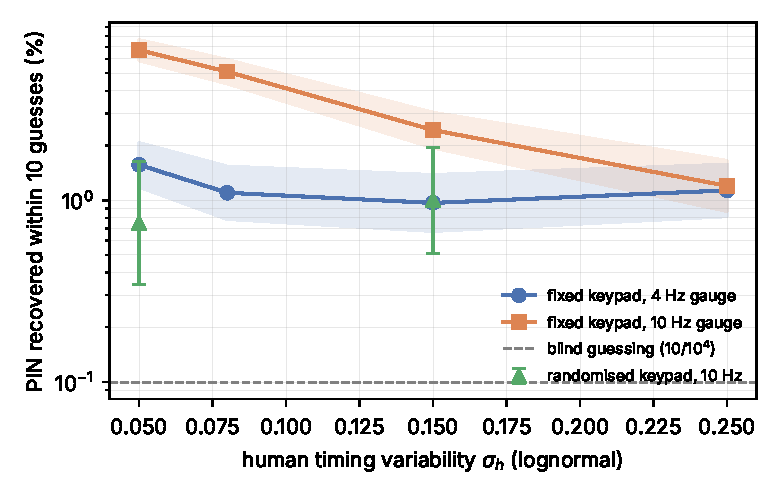
\includegraphics[width=0.72\linewidth]{fig_pin.pdf}
\caption{Probability of recovering a 4-digit PIN within ten guesses as a function of user timing variability. Shaded bands and error bars are 95\% Wilson intervals.}
\label{fig:pin}
\end{figure}

\paragraph{Results.} Table~\ref{tab:pin} and Figure~\ref{fig:pin} show three effects.
\begin{enumerate}
  \item \textbf{The channel is real but bounded by human noise.} On a fixed keypad at 10\,Hz, ten guesses succeed in about 3\% of entries for $\sigma_h{=}0.15$, a thirty-fold gain over blind guessing (0.1\%), and about 6.7\% for a very consistent user ($\sigma_h{=}0.05$, median rank 200). At 4\,Hz the gain is roughly ten-fold. This is far from the near-unique recovery suggested by the worked example in~\cite{gn23}, which used noiseless delays, but against an $L{=}10$ attempt limit it is a material increase in a thief's success probability.
  \item \textbf{Faster sampling helps little beyond 10\,Hz}, because human variability rather than quantization dominates: hit@10 rises only from 2.97\% to 3.38\% between 10 and 50\,Hz.
  \item \textbf{Randomized layouts remove distance information but not repetition.} With per-entry randomization, the attacker's posterior depends only on which digits repeat, and success returns close to the blind level. In a separate run of 600 randomized entries ($\sigma_h{=}0.05$, 10\,Hz), all three ten-guess successes were PINs containing a repeated digit; none of the 288 PINs with four distinct digits was found. A repeated digit produces a zero-distance interval regardless of layout. Rule R3 addresses this.
\end{enumerate}

\paragraph{Effect on Theorem~\ref{prop:pin}.} With $L{=}10$, a device thief who also has a fuel-gauge trace succeeds with roughly 3--7\% probability on a fixed keypad, versus about 0.1\% blind. With R1 the advantage is provably capped at 1.5\% for any observation of pressed keys (Corollary~\ref{cor:rand}), consistent with the simulated 0.67--1.0\%. With R1 and R3 it is exactly the blind rate. The device share's user-presence binding removes the scenario entirely when it is enforced, which is why R4 and keystore gating are part of the method rather than optional.

\paragraph{Model limitations.} The timing parameters are illustrative, not fitted to measured traces; real users have digit-specific habits that a profiled attacker could exploit, which would increase leakage on fixed keypads. We assume perfect press detection; disabling haptics (R2) makes detection harder in practice~\cite{gn23}. The model ignores gyroscope fusion, which~\cite{gn23} uses to sharpen timing and which can leak spatial information directly~\cite{taplogger12,berend17}. On-device measurement across devices is future work.

\section{Discussion}
\label{sec:split}

\paragraph{Why not threshold signing?} The cleanest embedded-wallet custody would let device and provider jointly authorize spends with FROST~\cite{frost20} while a delegated prover sees no spend secret. \SB{} binds spending to knowledge of $\sk_{\mathsf{spend}}$ inside the proof, so this requires a split of authority in the style of Zcash Sapling, where a proof-authorizing key enables proving and a re-randomized key signs a spend authorization outside the circuit~\cite{zcash}. Adding this to \SB{} would change the transfer statement and therefore require a new, non-interoperable deployment profile and setup~\cite[App.~A]{sb26}. It would also make M2-style delegated proving safe for custody, though not for privacy. We regard it as the most valuable protocol extension for embedded deployments and leave its specification and analysis to future work.

\paragraph{Viewing keys and compliance.} The \SB{} disclosure model already gives the user scoped read capabilities~\cite[§7]{sb26}. An embedded provider must not make $\vk_{\mathsf{in}}$ or $\vk_{\mathsf{out}}$ escrow a condition of service; when a regulated provider needs evidence, \textsc{NoteOpening} and \textsc{DerivedReport} disclosures, or the optional certified-recipient lineage of~\cite[App.~D]{sb26}, reveal less than a raw viewing key.

\paragraph{Liveness.} Every spend in \sysname{} requires $\mathcal{P}$'s HSM to release $\sigma_{\mathcal{P}}$, and M3 requires $\mathcal{P}$ online. If $\mathcal{P}$ disappears, the user recovers with $\{\sigma_{\mathcal{D}}, \sigma_{\mathcal{R}}\}$ and continues as a self-custodial \SB{} wallet; funds are never stranded by the provider, and anchor-window expiry only forces a rebuild, not a loss~\cite[§13]{sb26}.

\paragraph{Limitations.} The Rotom wrap's security reduces to Rotom-256 being a tweakable PRP. That is a cryptanalytic claim by its designers, not a proven property, and a masked Rotom implementation has not yet been evaluated~\cite[§5.4.2]{rotom26}; the cycle costs in §\ref{sec:hw} are summed from the designers' per-component figures rather than measured for the wrap itself. We do not measure on-device or MPC proving cost because the \SB{} circuit and curve parameters are not yet fixed. Our proofs reduce to the \SB{} theorem and to idealized models of the keystore (oracle access only) and of the PIN gate (an ideal functionality realized by an OPRF); attacks on these components, such as keystore extraction, are outside the proofs. The side-channel evaluation is a model, not a device experiment.

\section{Conclusion}
\SB{} specifies a private transfer layer for Bitcoin but leaves the wallet to the deployer. For embedded wallets, the decisive questions are where $\sk_{\mathsf{spend}}$ lives, who sees the witness, who learns which notes are whose, and how much the unlocking PIN leaks. \sysname{} answers them without touching the transfer statement: a 2-of-3 seed split with an attempt-limited OPRF PIN gate, on-device or collaborative proving, $k$-of-$n$ root agreement with delta download, local scanning by default, and side-channel-hardened PIN entry. The analysis shows that the largest risk is not cryptographic but organizational: a provider that scans and relays for its users can reconstruct their payment graph. The simulation shows that fuel-gauge leakage is modest but meaningful against attempt-limited PINs, and that keypad randomization neutralizes it except for repeated digits.


\appendix
\section{Simulation Details}
\label{app:sim}
This appendix gives the complete model behind Table~\ref{tab:pin} and Figure~\ref{fig:pin} so that the results can be reproduced.

\paragraph{Keypad.} Slots lie on a $4\times 3$ grid with unit pitch. Row $r \in \{0,1,2,3\}$ and column $c \in \{0,1,2\}$ give coordinates $(r,c)$. Digits $1$--$9$ occupy rows $0$--$2$ in reading order, digit $0$ is at $(3,1)$, \texttt{DEL} is at $(3,0)$, and \texttt{OK} is at $(3,2)$. In the ``randomized (digits)'' layout, the ten digits are permuted uniformly over their ten slots on each entry. In ``randomized (digits+OK)'', \texttt{OK} and \texttt{DEL} additionally swap positions with probability $1/2$.

\paragraph{Timing.} The interval between consecutive presses at Euclidean distance $D$ is $t = (a + b\log_2(1 + D/W))\cdot e^{\eta}$ with $a = 0.25$\,s, $b = 0.15$\,s/bit, $W = 1$, and $\eta \sim \mathcal{N}(0, \sigma_h^2)$ drawn independently for each interval. We use $\sigma_h \in \{0.05, 0.08, 0.15, 0.25\}$ and report $\sigma_h = 0.15$ in Table~\ref{tab:pin}.

\paragraph{Observation.} Press times are cumulative sums of the four intervals (digit$_1\!\to$digit$_2$, digit$_2\!\to$digit$_3$, digit$_3\!\to$digit$_4$, digit$_4\!\to$\texttt{OK}), starting at $0$. Each press is mapped to the index $\lfloor (t + \phi) f \rfloor$ of the fuel-gauge sample in which it falls, where $\phi \sim U[0, 1/f)$ is a random phase per entry and $f \in \{4, 10, 50\}$\,Hz. The adversary observes the four differences of consecutive indices.

\paragraph{Adversary.} For each distinct distance value, the likelihood of an observed index difference is estimated from $2\times 10^5$ Monte Carlo samples with independent phase, with a floor of $10^{-12}$ on empty bins. For the fixed layout, a PIN's log-likelihood is the sum over the four intervals, and all $10^4$ PINs are ranked under the uniform prior, with ties broken uniformly at random. For randomized layouts, the likelihood of each of the $15$ equality patterns is the average over $150$ sampled layouts. By Lemma~\ref{lem:pattern} this is the exact form of the Bayes-optimal likelihood, up to Monte Carlo error, and all PINs in a pattern share it.

\paragraph{Metrics and statistics.} For each entry we record the rank of the true PIN. Hit@$L$ is the fraction of entries with rank at most $L$. $2^{H}$ is the mean over entries of $2^{H(P)}$ for the posterior $P$. Confidence intervals are 95\% Wilson intervals. Trials per configuration are $4000$ (fixed layout, Table~\ref{tab:pin}), $3000$ (fixed layout, Figure~\ref{fig:pin}), and $300$ or $800$ (randomized). The pseudorandom generator is NumPy's \texttt{default\_rng} with seed $20261105$.

\section{Notation}
\label{app:notation}
\begin{center}\small
\begin{tabularx}{\linewidth}{@{}lX@{}}
\toprule
Symbol & Meaning \\
\midrule
$s = \seed$ & 32-byte wallet seed of \SB{} \\
$\sigma_{\mathcal{D}}, \sigma_{\mathcal{P}}, \sigma_{\mathcal{R}}$ & device, provider, and recovery shares of $s$ \\
$\pi$, $L$ & user PIN; HSM attempt limit \\
$\mathcal{F}_{\mathsf{gate}}$ & ideal PIN-gate functionality \\
$K_{\mathcal{D}}$, $K_{\mathsf{HW}}$ & keystore key (phone); chip-unique key (hardware variant) \\
$\varphi$ & address fingerprint for share-integrity checks \\
$\sk_{\mathsf{spend}}, \sk_{\mathsf{nf}}, \vk_{\mathsf{in}}, \vk_{\mathsf{out}}$ & \SB{} capabilities (Table~\ref{tab:caps}) \\
M1, M2, M3 & on-device, enclave, collaborative proving \\
V0, V1 & local and delegated scanning \\
R1--R4 & PIN-entry rules \\
W1--W3 & hardware-wrap rules \\
$\mathsf{RW}$, $\widetilde{E}$ & Rotom share wrap; Rotom-256 \\
$R[h]$, $R^\ast$ & replayed root at height $h$; correct root \\
$n, k$ & number of indexers queried; agreement threshold \\
$\mathsf{pat}(\pi)$ & equality pattern of a PIN \\
$G_L$ & device-theft success bound (Theorem~\ref{prop:pin}) \\
\bottomrule
\end{tabularx}
\end{center}

\begin{thebibliography}{99}\small
\bibitem{sb26} C.~Shikhelman, M.~Komarov, A.~Moskvin. \emph{Shielded Bitcoin: Private Transfers on the Bitcoin L1}. Cryptology ePrint Archive, Paper 2026/2749, 2026.
\bibitem{gn23} V.~Giraud, D.~Naccache. \emph{Bypassing Android isolation with fuel gauges: new risks with advanced power ICs}. Cryptology ePrint Archive, Paper 2023/1078, 2023.
\bibitem{gg18} R.~Gennaro, S.~Goldfeder. Fast multiparty threshold ECDSA with fast trustless setup. In \emph{ACM CCS}, 2018.
\bibitem{frost20} C.~Komlo, I.~Goldberg. FROST: Flexible round-optimized Schnorr threshold signatures. In \emph{Selected Areas in Cryptography (SAC)}, 2020.
\bibitem{opaque18} S.~Jarecki, H.~Krawczyk, J.~Xu. OPAQUE: An asymmetric PAKE protocol secure against pre-computation attacks. In \emph{EUROCRYPT}, 2018.
\bibitem{shamir79} A.~Shamir. How to share a secret. \emph{Communications of the ACM}, 22(11), 1979.
\bibitem{ob22} A.~Ozdemir, D.~Boneh. Experimenting with collaborative zk-SNARKs: Zero-knowledge proofs for distributed secrets. In \emph{USENIX Security}, 2022.
\bibitem{fmd21} G.~Beck, J.~Len, I.~Miers, M.~Green. Fuzzy message detection. In \emph{ACM CCS}, 2021.
\bibitem{zcash} D.~Hopwood, S.~Bowe, T.~Hornby, N.~Wilcox. \emph{Zcash Protocol Specification}. Electric Coin Company, 2016--2025.
\bibitem{rotom26} K.~Morita, K.~Minematsu, K.~Sakamoto, K.~Taka, R.~Ueno, T.~Isobe. \emph{Rotom: A Microcontroller-Oriented Tweakable Block Cipher Using Modular Multiplication} (full version). Cryptology ePrint Archive, Paper 2026/2693, 2026.
\bibitem{lrw02} M.~Liskov, R.~L.~Rivest, D.~Wagner. Tweakable block ciphers. In \emph{CRYPTO}, 2002.
\bibitem{kr11} T.~Krovetz, P.~Rogaway. The software performance of authenticated-encryption modes. In \emph{FSE}, 2011.
\bibitem{fitts54} P.~M.~Fitts. The information capacity of the human motor system in controlling the amplitude of movement. \emph{Journal of Experimental Psychology}, 47(6), 1954.
\bibitem{sd03} A.~Serjantov, G.~Danezis. Towards an information theoretic metric for anonymity. In \emph{Privacy Enhancing Technologies (PET 2002)}, LNCS 2482, Springer, 2003.
\bibitem{taplogger12} Z.~Xu, K.~Bai, S.~Zhu. TapLogger: Inferring user inputs on smartphone touchscreens using on-board motion sensors. In \emph{ACM WiSec}, 2012.
\bibitem{berend17} D.~Berend, B.~Jungk, S.~Bhasin. There goes your PIN: Exploiting smartphone sensor fusion under single and cross user setting. Cryptology ePrint Archive, Paper 2017/1169, 2017.
\end{thebibliography}

\end{document}
